\documentclass{article}
\usepackage{graphicx}
\usepackage{amsmath}
\usepackage{hyperref}
\usepackage{listings}
\usepackage{float}

\usepackage{color}
\definecolor{lightgray}{rgb}{.9,.9,.9}
\definecolor{darkgray}{rgb}{.4,.4,.4}
\definecolor{purple}{rgb}{0.65, 0.12, 0.82}

\lstdefinelanguage{JavaScript}{
  keywords={typeof, new, true, false, catch, function, return, null, catch, switch, var, if, in, while, do, else, case, break},
  keywordstyle=\color{blue}\bfseries,
  ndkeywords={class, export, boolean, throw, implements, import, this},
  ndkeywordstyle=\color{darkgray}\bfseries,
  identifierstyle=\color{black},
  sensitive=false,
  comment=[l]{//},
  morecomment=[s]{/*}{*/},
  commentstyle=\color{purple}\ttfamily,
  stringstyle=\color{red}\ttfamily,
  morestring=[b]',
  morestring=[b]"
}

\lstset{
   language=JavaScript,
   backgroundcolor=\color{lightgray},
   extendedchars=true,
   basicstyle=\footnotesize\ttfamily,
   showstringspaces=false,
   showspaces=false,
   numbers=left,
   numberstyle=\footnotesize,
   numbersep=9pt,
   tabsize=2,
   breaklines=true,
   showtabs=false,
   captionpos=b
}

\title{%
Howework 1 \\
\large Interactive Graphics}

\date{May 2018}
\author{Ibis Prevedello}

\begin{document}
\maketitle

\section{Introduction}
The goal of this homework is to use WebGL with control code written in JavaScript in order to draw an interactive 3D Cube in an HTML canvas in a web browser. The source code for this project can be accessed from my \href{https://github.com/ibiscp/Computer-Graphics-WebGL}{GitHub page}.

\section{Development}
A series of improvements were done in the base code in order to achieve the following effects:

\begin{enumerate}
\item Add a button that changes the direction of the current rotation.
\item Move the transformations matrices from the shader to the Javascript application, so that the ModelView and Projection matrix are computed in the application and then transferred to the shader.
\item Include a scaling (uniform, all parameters have the same value) and a translation Matrix and control them with sliders.
\item Define an orthographic projection with the planes near and far controlled by sliders.
\item Define a perspective projection, introduce a button that switches between orthographic and perspective projection. The slider for near and far should work for both projections.
\item Introduce a light source, replace the colors by the properties of the material (your choice) and assign to each vertex a normal.
\item Implement both the Gouraud and the Phong shading models, with a button switching between them.
\end{enumerate}

\subsection {Item 1 - Change rotation direction}
For the implementation of this item, it is necessary only to decrement the value of the angle instead of increment it, based on a variable chosen by the user.

\begin{lstlisting}[language=JavaScript]
if(direction)
  theta[axis] += 2.0;
else
  theta[axis] -= 2.0;}
\end{lstlisting}

\subsection {Item 2 - Move the transformation matrices}
In order to move the transformation matrices from the \textit{shader} to the \textit{JavaScript} application it was implemented multiplying the matrices as shown below.

\begin{lstlisting}[language=JavaScript]
modelViewMatrix = lookAt(eye, at, up);
modelViewMatrix = mult(modelViewMatrix,
    rotate(theta[xAxis], [1, 0, 0]));
modelViewMatrix = mult(modelViewMatrix,
    rotate(theta[yAxis], [0, 1, 0]));
modelViewMatrix = mult(modelViewMatrix,
    rotate(theta[zAxis], [0, 0, 1]));
gl.uniformMatrix4fv(gl.getUniformLocation(program,
    "modelViewMatrix"), false, flatten(modelViewMatrix));
\end{lstlisting}

\subsection {Item 3 - Include scaling and translation}
For the scaling and translation matrix it is possible to use the same functions in the \textit{modelViewMatrix}.

\begin{lstlisting}[language=JavaScript]
modelViewMatrix = lookAt(eye, at, up);
modelViewMatrix = mult(modelViewMatrix,
    scalem(sliderScale, sliderScale, sliderScale));
modelViewMatrix = mult(modelViewMatrix,
    translate(sliderTX, sliderTY, sliderTZ));
modelViewMatrix = mult(modelViewMatrix,
    rotate(theta[xAxis], [1, 0, 0]));
modelViewMatrix = mult(modelViewMatrix,
    rotate(theta[yAxis], [0, 1, 0]));
modelViewMatrix = mult(modelViewMatrix,
    rotate(theta[zAxis], [0, 0, 1]));
gl.uniformMatrix4fv(gl.getUniformLocation(program,
    "modelViewMatrix"), false, flatten(modelViewMatrix));
\end{lstlisting}

\subsection {Item 4 - Orthographic projection}
For the orthographic projection it is possible to implement using the function \textit{ortho}.

\begin{lstlisting}[language=JavaScript]
projectionMatrix = ortho(left, right, bottom, ytop, near, far); 
gl.uniformMatrix4fv(gl.getUniformLocation(program,
    "projectionMatrix"), false, flatten(projectionMatrix));
\end{lstlisting}

\subsection {Item 5 - Perspective projection}
For this item it is also necessary to be possible to change the projection with a button. For this case the projection can be changed based on a flag and the projection changed between orthogonal and perspective.

\begin{lstlisting}[language=JavaScript]
if(perspec)
    projectionMatrix = perspective(fovy, aspect, near, far);
else
    projectionMatrix = ortho(left, right, bottom, ytop, near, far);
    gl.uniformMatrix4fv(gl.getUniformLocation(program,
        "projectionMatrix"), false, flatten(projectionMatrix));
\end{lstlisting}

\subsection {Item 6 - Introducing the light source}
For the light source, it is a little bit more complex because some more serious modification is necessary.

First, it is necessary to define light position, and ambient, diffuse and specular lights as well as material and shininess. This variables are passed to the \textit{shader} and there they are used to create the light effect. Because this piece of code is a little more complex, it will not be showed here, but the full code can be found in my GitHub repository.

\subsection {Item 7 - Gouraud and Phong shading models}
For the Gouraud and Phong shading models, both are implemented in the \textit{shader}, a button was added to make it possible to change from one model to another. Because the code is also a little bit complex, it can be verified in my GitHub repository.

One of the things that were not mentioned here is the process to create the vertex normals, for the normals it is possible to create it manually, what is not difficult for the case of a cube, however, for more complex models it becomes impossible. So, it can be added to the function \textit{quad} and the normals are created automatically, as shown below.

\begin{lstlisting}[language=JavaScript]
var t1 = subtract(vertices[b], vertices[a]);
var t2 = subtract(vertices[c], vertices[b]);
var normal = cross(t1, t2);
var normal = vec3(normal);
normal = normalize(normal);
\end{lstlisting}

\section{Conclusion}
After implement all the features it was possible to see the evolution of the cube as more features were being added, reaching the final result of a real realistic cube, with perspective and lightning, compared with the base code.

\begin{figure}[!ht]
\centering
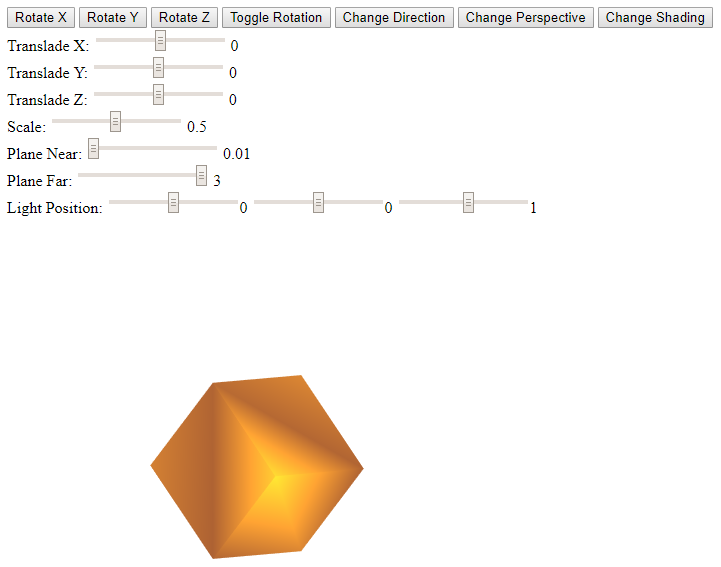
\includegraphics[scale=0.50]{cube3d}
\caption{Cube 3D screenshot}
\label{fig:fig1}
\end{figure}

\end{document}